\section{Characterization of 3-planar graphs}
\label{sec:3planar}

Let $G$ be an optimal $3$-planar graph on $n$ vertices (and therefore with $5.5n-11$ edges) and let $\Gamma(G)$ be a PMCM $3$-planar drawing of $G$, i.e. $\Gamma(G)$ has the maximum number of true-planar edges among all potential $3$-planar drawing of $G$ and, subject to this restriction, $\Gamma(G)$ has also the minimum number of crossings. 
As in the previous section, we will initially assume that in the drawing $\Gamma(G)$ there is no pair of edges that cross twice, i.e. $\Gamma(G)$ is almost-simple. In Lemma~\ref{lem:3_planar_cross_twice} we will formally prove that indeed all PMCM drawings are also almost-simple. In the following we examine structural properties of an almost-simple PMCM drawing $\Gamma(G)$, in particular we show  that the true planar skeleton $\Pi(G)$ of $\Gamma(G)$ consists of faces of length at most $9$. 

\begin{lemma}\label{lem:no-of-edges}
Let $f_s$ be a facial $s$-cycle of $\Pi(G)$ of a PMCM $3$-planar drawing of an optimal $3$-planar graph $G$. Then, for $6\leq s\leq 10$ $f_s$ cannot contain more than $c(s)$ chords drawn entirely in its interior (see Figure~\ref{fig:replacements}), where:\todo{Do we assume almost-simple as we state few lines above? This should be clear in each lemma, e.g., in Lemma~\ref{lem:size9}.}

$c(s)=\left\{
\begin{array}{ll}
8,  &s=6\\
9,  &s=7\\
11, &s=8\\
14, &s=9\\
17, &s=10\\
\end{array}
\right.
$
\end{lemma}
\begin{proof}
For $6\leq s\leq 10$, if $f_s$ contains strictly more than $c(s)$ chords in its interior, then one can observe that at least one chord of $f_s$ has $4$ crossings or more. On the other hand, Figure~\ref{fig:replacements} is a certificate that $f_s$ can indeen contain $c(s)$ chords without violating $3$-planarity. This completes the proof of this lemma.
\end{proof}

\begin{figure}[thb]
    \centering
    \begin{minipage}[b]{.18\textwidth}
        \centering
        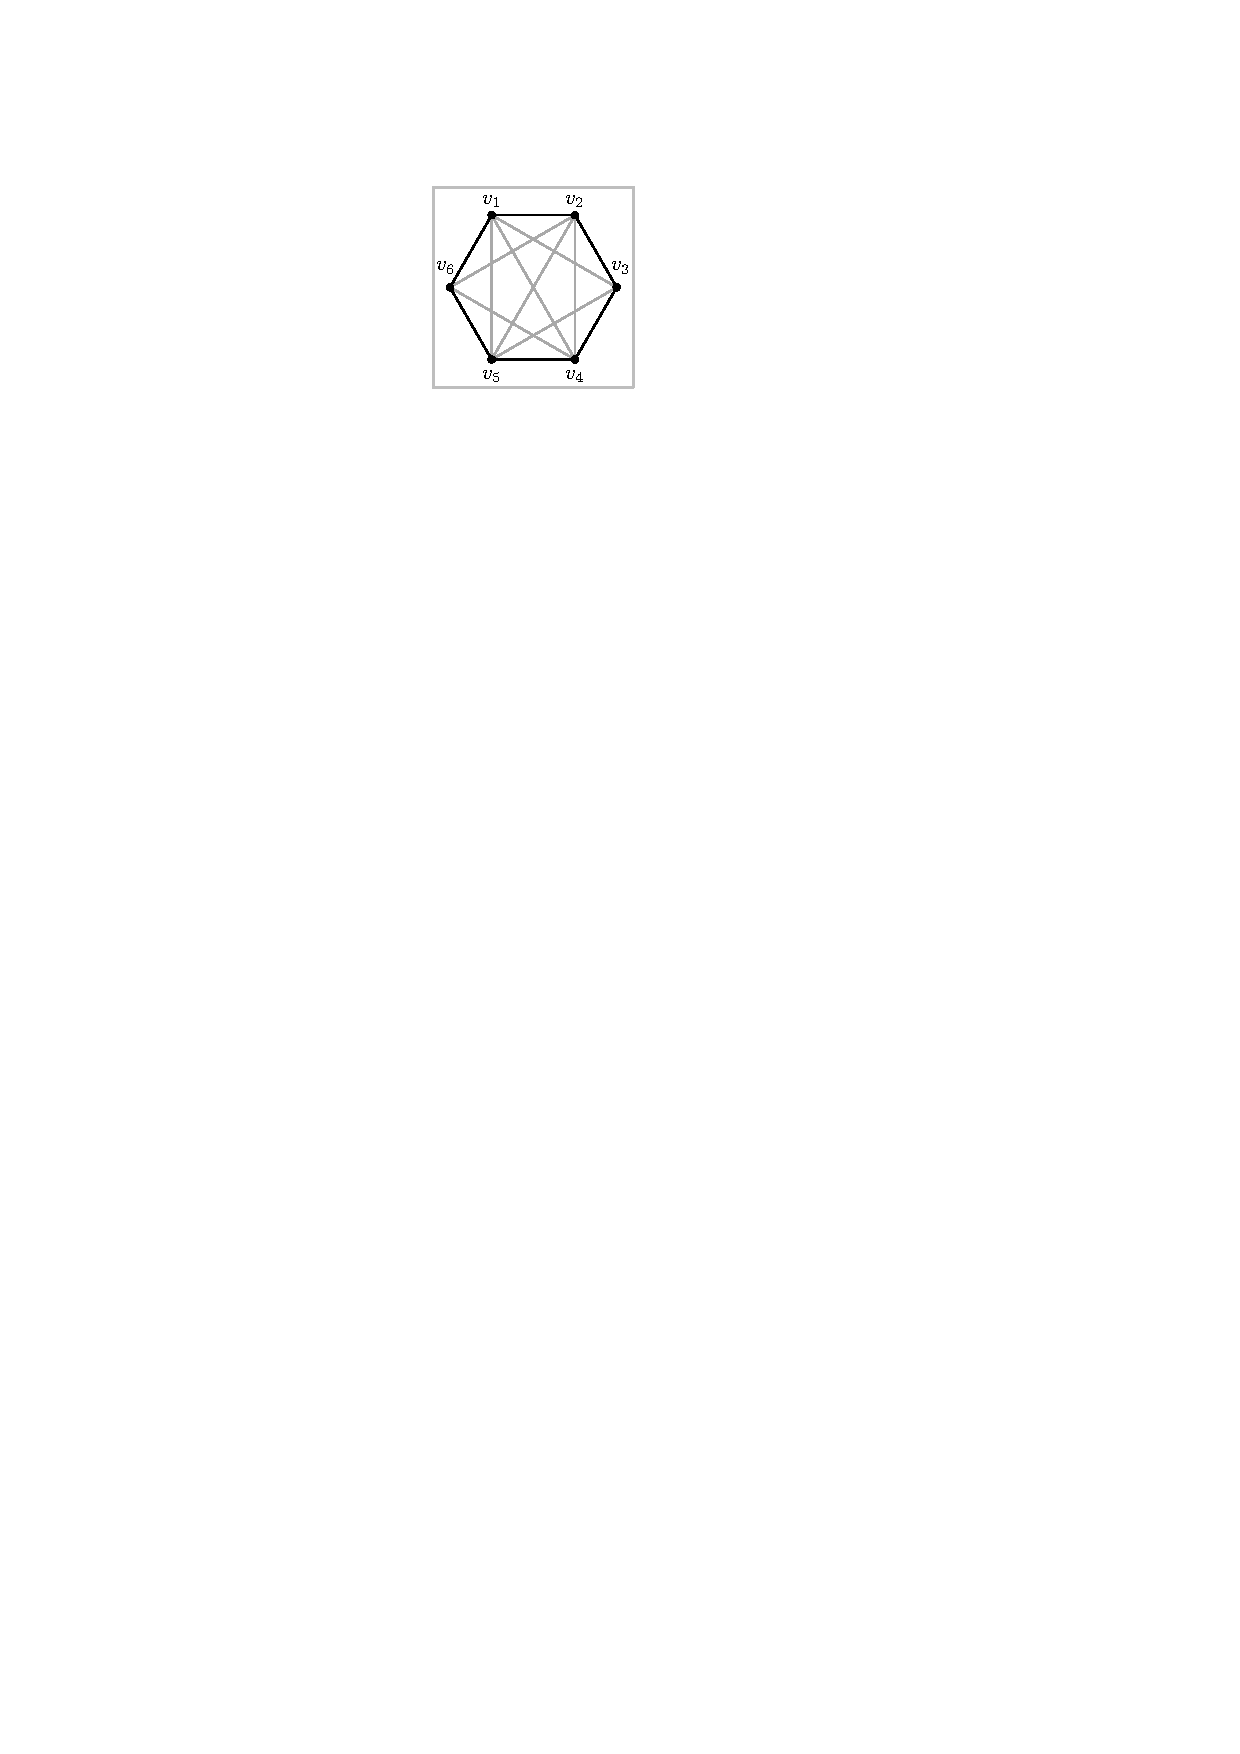
\includegraphics[width=\textwidth,page=1]{images/polygon_conf}
        \subcaption{$s=6$}\label{fig:6gon}
    \end{minipage}
    \begin{minipage}[b]{.18\textwidth}
        \centering
        \includegraphics[width=\textwidth,page=2]{images/polygon_conf}
        \subcaption{$s=7$}\label{fig:7gon}
    \end{minipage}
    \begin{minipage}[b]{.18\textwidth}
        \centering
        \includegraphics[width=\textwidth,page=3]{images/polygon_conf}
        \subcaption{$s=8$}\label{fig:8gon}
    \end{minipage}
    \begin{minipage}[b]{.18\textwidth}
        \centering
        \includegraphics[width=\textwidth,page=4]{images/polygon_conf}
        \subcaption{$s=9$}\label{fig:9gon}
    \end{minipage}
    \begin{minipage}[b]{.18\textwidth}
        \centering
        \includegraphics[width=\textwidth,page=5]{images/polygon_conf}
        \subcaption{$s=10$}\label{fig:10gon}
    \end{minipage}
    \caption{%
    Configurations of Lemma~\ref{lem:no-of-edges}.}
    \label{fig:replacements}
\end{figure}

In the following we consider a \pp $\mathcal{C}_s$ of $s$ vertices in $\Gamma(G)$, where $6\leq s\leq 9$. Let $E_s$ be the set of edge-segments that pass through the interior of $\mathcal{C}_s$. Note that $E_s$ may contain also edges that are chords of $\mathcal{C}_s$. We call $E_s$ the \emph{passing-through segments} of $\mathcal{C}_s$. 

\begin{lemma}
Let $\Gamma(G)$ be a PMCM $3$-planar drawing of an optimal $3$-planar graph $G$, and let $s$ such that $6\leq s\leq 9$. Suppose that there exists a \pp $\mathcal{C}_s$ of $s$ vertices in $\Gamma(G)$, such that the potential boundary edges of $\mathcal{C}_s$ belong in $\Gamma(G)$. Let $E_s$ be the set of passing-through segments of $\mathcal{C}_s$. If the following conditions hold, then there exists an empty true-planar $s'$-cycle $\mathcal{C}_{s'}$ in $\Gamma(G)$, with $s\leq s'\leq 9$, and all edges with edge-segments in $E_s$ are drawn as chords in its interior.
\begin{enumerate}[C.1:]
\item $|E_s|\leq 2s-4$, and, 
\item every edge-segment of $E_s$ has at least one crossing in the interior of $\mathcal{C}_s$.
\end{enumerate}
\label{lem:size9}
\end{lemma}

\begin{proof}
We start with the following observation: At most one edge-segment of an edge $e$ belongs to $E_s$. This is true, because of $3$-planarity. In particular, if $E_s$ contains at least two edge-segments of $e$, then we claim that $e$ has at least four crossings. By Condition C.2 each of the two edge-segments of $e$ contributes one crossing to $e$. Since $\mathcal{C}_s$ is empty and contains two edge-segments of $e$, it follows that $e$ enters and exits $\mathcal{C}_s$. Hence $e$ has two more crossings, suming up to a total of at least four crossings. 

To prove the lemma, we employ a backward inductive proof. First, we prove that the lemma holds for the base case where $s=9$. Let $v_1,v_2,\dots,v_9$ be the vertices of $\mathcal{C}_s$ in this case. If all edges with edge-segments in $E_s$ completely lie in $\mathcal{C}_s$,  then $\mathcal{C}_s$ is a true-planar $s$-cycle, and the lemma holds for $s'=s$. Otherwise, there is at least one edge $e$ with an edge-segment in $E_s$, that crosses an edge of $\mathcal{C}_s$ (refer to Figure~\ref{fig:cs1}). W.l.o.g.~we can assume that $e$ crosses edge $(v_1,v_9)$ of $\mathcal{C}_s$ at point $c$. If $w$ and $w'$ are the two endpoints of $e$, then by the observation we made at the beginning of the proof it follows that either edge-segment $(w,c)$ or edge-segment $(c,w')$ of $e$ is entirely drawn outside $\mathcal{C}_s$ (as otherwise $e$ would have at least two edge-segments in $E_{s}$). W.l.o.g.~assume that edge-segment $(w,c)$ of $e$ is drawn outside $\mathcal{C}_s$. Then corner edges $[v_1,w]$ and $[w,v_9]$ are \pes (by Property~\ref{prp:corner}). 

\begin{figure}[t!]
    \centering
    \begin{minipage}[b]{.19\textwidth}
        \centering
        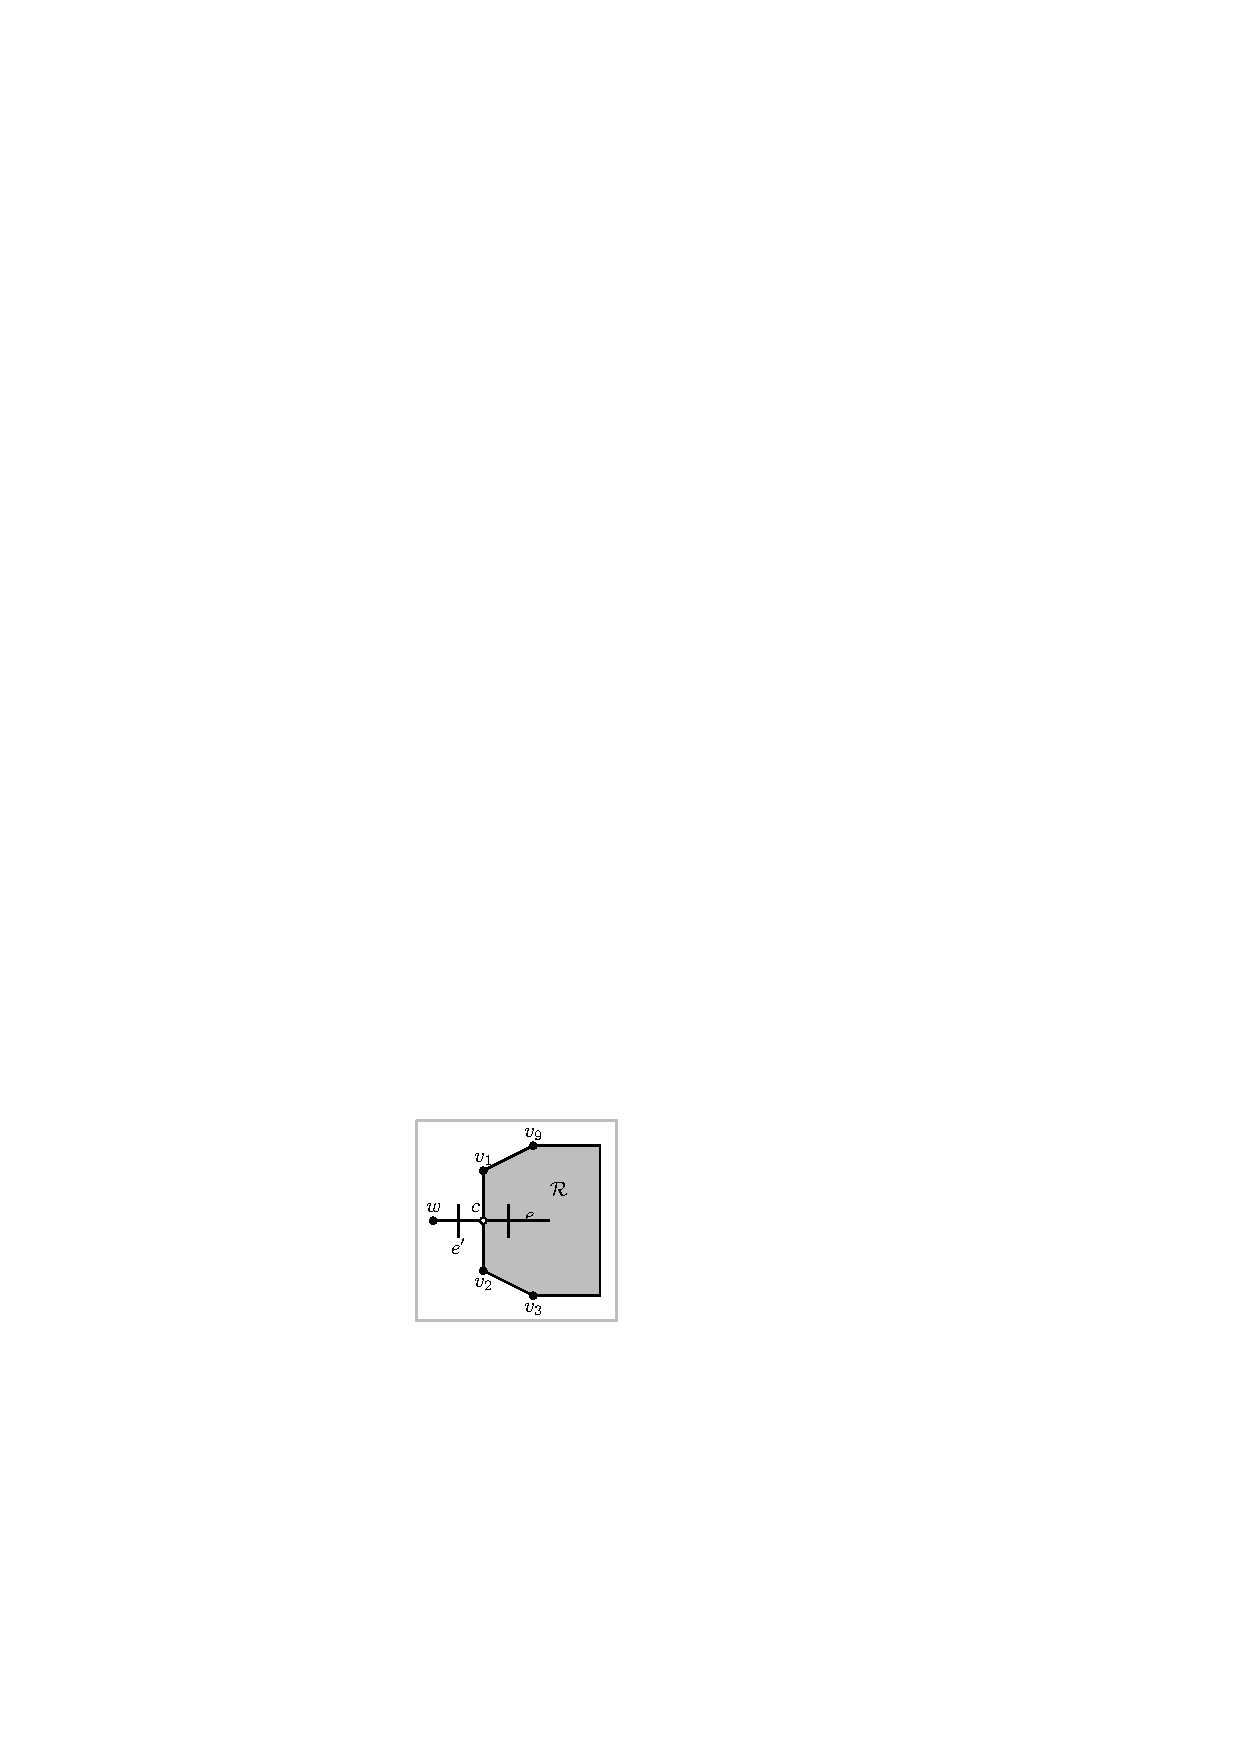
\includegraphics[width=\textwidth,page=1]{images/3planar_polygon}
        \subcaption{~}\label{fig:cs1}
    \end{minipage}
    \begin{minipage}[b]{.19\textwidth}
        \centering
        \includegraphics[width=\textwidth,page=2]{images/3planar_polygon}
        \subcaption{~}\label{fig:cs2}
    \end{minipage}
	\begin{minipage}[b]{.19\textwidth}
        \centering
        \includegraphics[width=\textwidth,page=6]{images/polygon_conf}
        \subcaption{~}\label{fig:7_stick}
    \end{minipage}
    \begin{minipage}[b]{.19\textwidth}
        \centering
        \includegraphics[width=\textwidth,page=7]{images/polygon_conf}
        \subcaption{~}\label{fig:8_stick}
    \end{minipage}
    \begin{minipage}[b]{.19\textwidth}
        \centering
        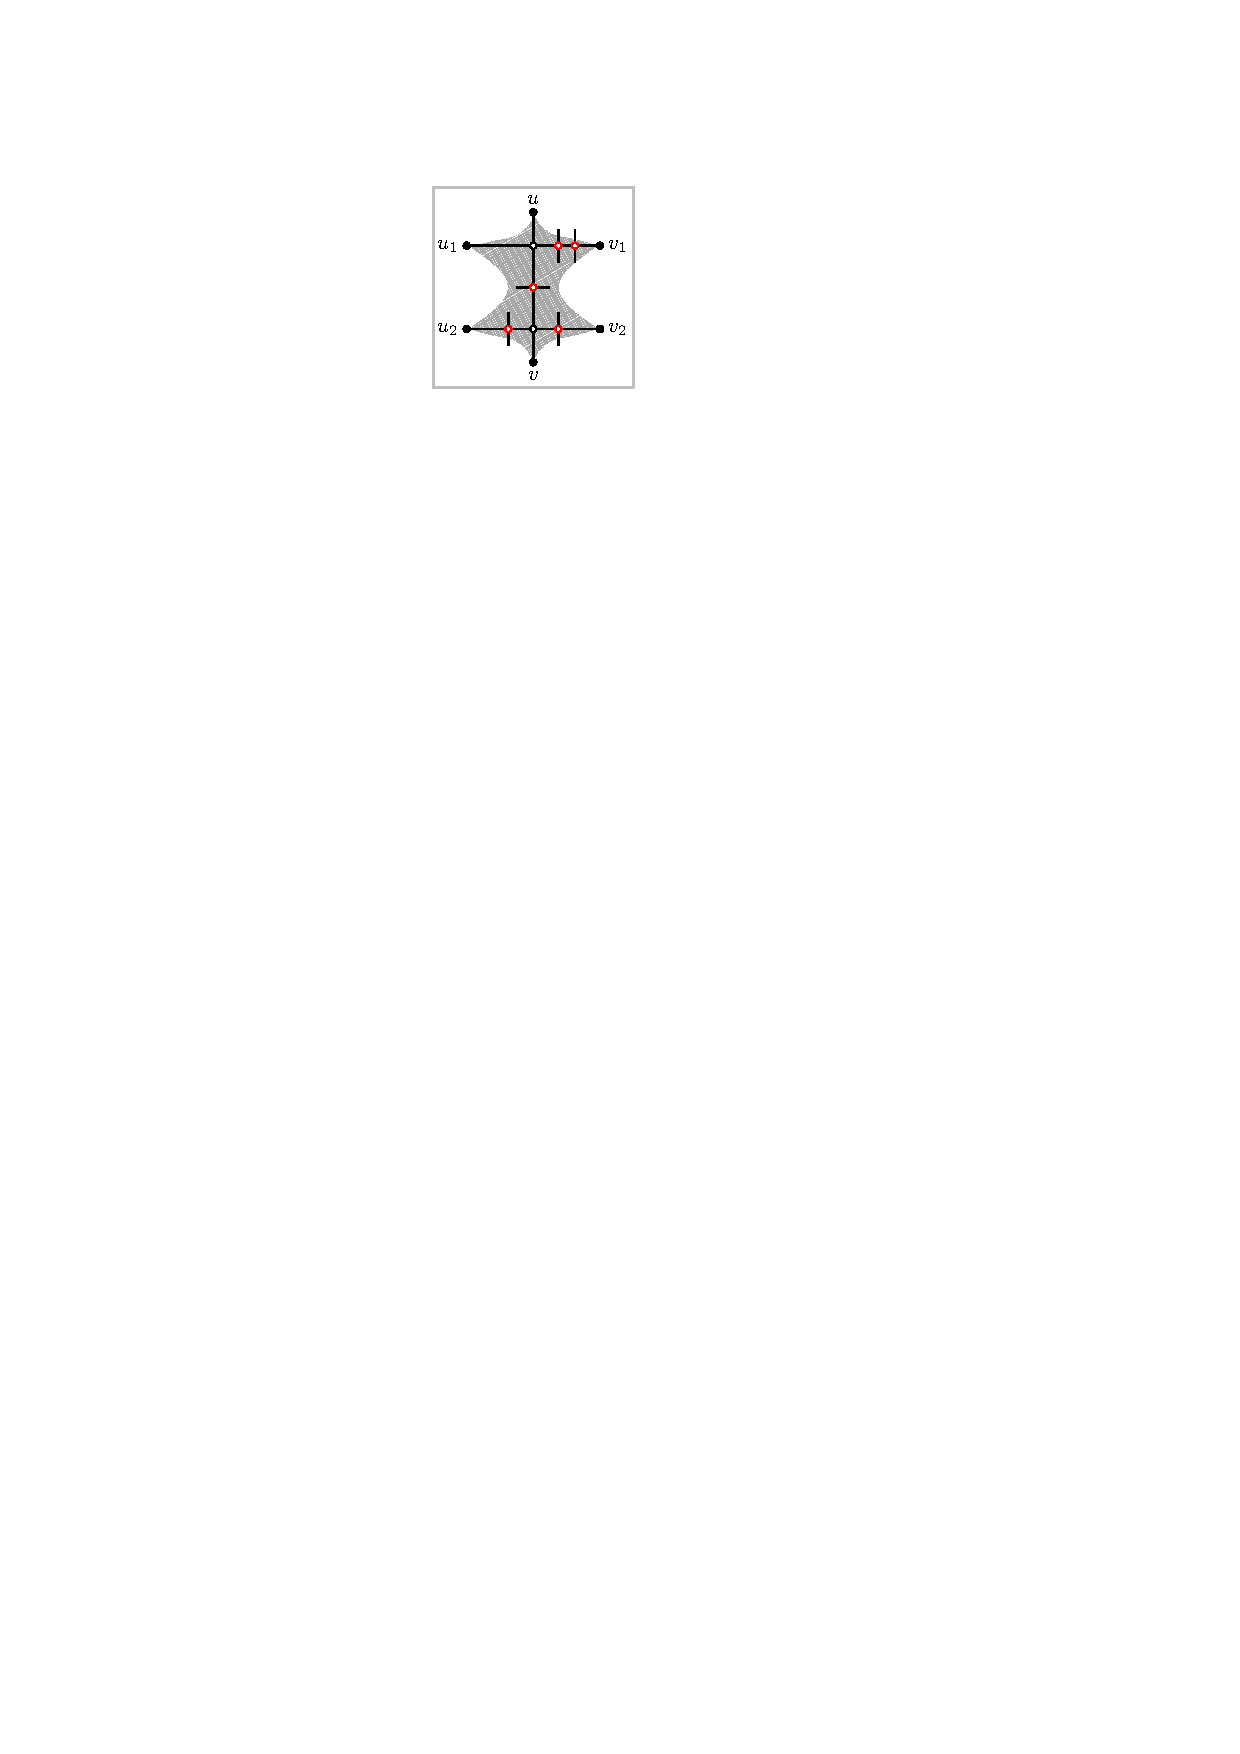
\includegraphics[width=\textwidth,page=1]{images/3planar_independent}
        \subcaption{~}\label{fig:independent}
    \end{minipage}
    \caption{%
    Different configurations used in  
    (a)-(d)~Lemma~\ref{lem:size9}, 
    (e)~Lemma~\ref{lem:3_planar_independent}.}
    \label{fig:replacements_2}
\end{figure}

Recall that edge $e$ has one crossing in the interior of $\mathcal{C}_s$ (by Condition C.2 of the lemma) and one more crossing with edge $(v_1,v_9)$. By $3$-planarity, it follows that edge $e$ may have at most one more crossing, say with edge $e'$. Note that $e'$ may have an edge-segment in $E_s$. Vertices $w,v_1,v_2,\dots,v_9$ define a \pp $\mathcal{C}_{s'}$ on $10$ vertices (see Figure~\ref{fig:cs2}). The set of passing-through segments $E_{s'}$ of $\mathcal{C}_{s'}$ contains all edge-segments of $E_s$ (that is, $E_s \subseteq E_{s'}$) plus at most two additional edge-segments: the one defined by edge $(v_1,v_9)$, and possibly an edge-segment of $e'$. By Condition C.1 of the lemma it follows that $|E_s| \leq 14$. Hence, $|E_{s'}| \leq 16$. However, we can replace $E_{s'}$ with the $3$-planar crossing pattern of Figure~\ref{fig:10gon} which contributes $17$ edges in $\Gamma(G)$. So, the derived graph has more edges than $G$, which is a contradiction to the optimality of $G$. Hence, for the case where $s=9$, we can conclude that $\mathcal{C}_s$ is indeed an empty true-planar cycle and additionally all edges with edge-segment in $E_s$ completely lie in $\mathcal{C}_s$.

For the inductive hypothesis, assume that the lemma holds for $6<s\leq 9$. We will prove that it also holds for $s-1$. So, let $v_1,v_2,\dots,v_{s-1}$ be the vertices of $\mathcal{C}_{s-1}$. As in the base case, if all edges with edge-segments in $E_{s-1}$ completely lie in $\mathcal{C}_{s-1}$, then $\mathcal{C}_{s-1}$ is clearly a true-planar $(s-1)$-cycle, and the lemma holds for $s'=s-1$. Otherwise, there is at least one edge $e$ with an edge-segment in $E_{s-1}$, that crosses an edge of $\mathcal{C}_{s-1}$. W.l.o.g.~assume that $e$ crosses edge $(v_1,v_{s-1})$ of $\mathcal{C}_s$ at point $c$. Let $w$ and $w'$ be the endpoints of $e$. As in the base case, we will assume that edge-segment $(w,c)$ of $e$ is drawn outside $\mathcal{C}_s$. Hence, by Property~\ref{prp:corner} corner edges $[v_1,w]$ and $[w,v_{s-1}]$ are \pes.

Similar to the base case, edge $e$ has one crossing in the interior of $\mathcal{C}_{s-1}$ (by Condition C.2 of the lemma) and one more crossing with edge $(v_1,v_{s-1})$. By $3$-planarity, edge $e$ may have at most one more crossing, say with edge $e'$, which may also have an edge-segment in $E_s$. On the other hand, vertices $w,v_1,v_2,\dots,v_{s-1}$ define a \pp $\mathcal{C}_{s}$ on $s$ vertices. The set of passing-through segments $E_{s}$ of $\mathcal{C}_{s}$ contains all edge-segments of $E_{s-1}$ (that is, $E_{s-1} \subseteq E_s$) plus at most two additional edge-segments: the one defined by edge $(v_1,v_{s-1})$, and possibly an edge-segment of $e'$. By Condition C.1 of the lemma, it follows that $|E_{s-1}| \leq 2(s-1)-4$. Hence, $|E_{s}| \leq 2s-4$, which implies that $\mathcal{C}_{s}$ satisfies Condition C.1 of the lemma. We now claim that Condition C.2 is also satisfied. Indeed, all edge-segments of $E_{s-1}$ have at least one crossing in the interior of $\mathcal{C}_s$ (recall that $E_{s-1}\subset E_s$). Since $(v_1,v_{s-1})$ and $e'$ both cross $e$ in the interior of $\mathcal{C}_s$, it follows that the remaining edge-segments of $\mathcal{C}_s$ (i.e., the ones defined by edges $(v_1,v_{s-1})$ and $e'$) have at least one crossing in the interior of $\mathcal{C}_s$. Hence, Condition C.2 is also satisfied. 

Since $6<s\leq 9$ and $|E_{s}| \leq 2s-4$, it is not hard to see that $|E_s|\leq c(s)+1$ also holds, where $c(s)$ is the number of edges defined in Lemma~\ref{lem:no-of-edges}. We distinguish two cases:% 
\begin{inparaenum}[(i)]
\item $|E_s|\leq c(s)$, or 
\item $|E_s|= c(s)+1$.
\end{inparaenum}
In both cases, we seek to show that the edges of $\mathcal{C}_s$ exist (up to homotopy\todo{Is it clear?}) in $\Gamma(G)$. In the former case, we proceed by replacing all edges with edge-segments in $E_s$ with the corresponding $3$-planar crossing pattern of Figure~\ref{fig:replacements} which contributes exactly $c(s)$ edges in $\Gamma(G)$. So, the derived graph has at least as many edges as $G$. However, since $G$ is optimal, it follows that all boundary edges of $\mathcal{C}_s$ must exist in $\Gamma(G)$. Consider now the later case, where $|E_s|= c(s)+1$. This case can occur only if $s=7$ or $s=8$. Additionally there must exist at least one edge with an edge-segment in $E_s$ that is not drawn entirely in the interior of $\mathcal{C}_s$. In other words, this particular edge must cross a boundary edge of $\mathcal{C}_s$, say at point $c$. We proceed by replacing all edges with edge-segments in $E_s$ with the $3$-planar crossing pattern of Figure~\ref{fig:7_stick} or~\ref{fig:8_stick} (depending on whether $s=7$ or $s=8$, respectively), which contributes exactly $c(s)+1$ edges in $\Gamma(G)$. Note that the end-point of each of the bold-drawn edges of Figures~\ref{fig:7_stick} and~\ref{fig:8_stick} that does not belong to $\mathcal{C}_s$ is identified with one of the end-points of the corresponding edge with the edge-segment in $E_s$ that is not drawn entirely in the interior of $\mathcal{C}_s$. Hence, $3$-planarity is preserved and the derived graph has at least as many edges as $G$. Since $G$ is optimal, it follows that all boundary edges of $\mathcal{C}_s$ must exist in $\Gamma(G)$.

In both cases the vertices of $\mathcal{C}_s$ define an empty $s$-cycle in $\Gamma(G)$ and $E_s$ satisfies the two conditions of the lemma as mentioned earlier. Hence, by the induction hypothesis, there exists a true planar cycle on $s'$ vertices, where $s\leq s'\leq 9$, with all edge-segments of $E_s$, and therefore of $E_{s-1}$,  as chords.
\end{proof}

%Suppose that in almost-simple PMCM drawing $\Gamma(G)$ of graph $G$ an edge $e$ is crossed by two edges $e_1$ and $e_2$, where $e_i=(u_i,v_i)$ for $i=1,2$. Recall that if $\Gamma(G)$ is almost-simple then at least one of parallel edges $[u_1,u_2]$ and $[v_1,v_2]$ is a \pe of $\Gamma(G)$. Also, in the case where both parallel edges $[u_1,u_2]$ and $[v_1,v_2]$ are \pes of $\Gamma(G)$, $e_1$ and $e_2$ are called independent.

Let $(u,v)$ be an edge of $G$ that is crossed by two edges $(u_1,v_1)$ and $(u_2,v_2)$ in $\Gamma(G)$. Since $\Gamma(G)$ is almost-simple, by Property~\ref{prp:parallel} it follows that at least one of parallel edges $[u_1,u_2]$ and $[v_1,v_2]$ is a \pe of $\Gamma(G)$. Recall that in the case where both parallel edges $[u_1,u_2]$ and $[v_1,v_2]$ are \pes of $\Gamma(G)$, edges $(u_1,v_1)$ and $(u_2,v_2)$ are called independent.

\begin{lemma}\label{lem:3_planar_independent}
Let $\Gamma(G)$ be an almost-simple PMCM $3$-planar drawing of an optimal $3$-planar graph~$G$. If edge $(u,v)$ is crossed by two independent edges $(u_1,v_1)$ and $(u_2,v_2)$, then $(u,v)$ is a chord of an empty true-planar $s$-cycle, where $6\leq s\leq 9$.
\end{lemma}
\begin{proof}
Refer to Figure~\ref{fig:independent}. Since $(u_1,v_1)$ and $(u_2,v_2)$ are independent edges, both parallel edges $[u_1,u_2]$ and $[v_1,v_2]$ are \pes. By Property~\ref{prp:corner}, it follows that corner edges $[u, u_1]$, $[u,v_1]$, $[u,u_2]$ and $[v,v_2]$ are also potential edges. Hence, vertices $u$, $u_1$, $u_2$, $v$, $v_2$ and $v_1$ define a \pp $\mathcal{C}$ on six vertices (gray-shaded in Figure~\ref{fig:independent}). Let $E$ be the set of passing-through edges of $\mathcal{C}$. We claim that $|E|\leq 8$. Indeed, set $E$ contains edges $(u,v)$, $(u_1,v_1)$, $(u_2,v_2)$, at most one other edge that crosses $(u,v)$, and at most four other edges that cross $(u_1,v_1)$ or $(u_2,v_2)$. We proceed by removing all edges of $E$ from $\Gamma(G)$ and replace them with the $3$-planar crossing pattern of Figure~\ref{fig:6gon}. In the derived drawing there exist $8$ edges that are drawn in the interior of $\mathcal{C}$ (without crossing $\mathcal{C}$). Since $G$ is optimal, it follows that $|E|=8$ and additionally all boundary edges of $\mathcal{C}$ exist in $\Gamma(G)$. Since $|E|=8$, all edges of $E$ have at least one crossing in the interior of $\mathcal{C}$. So, by Lemma~\ref{lem:size9} there exists an empty true-planar $s$-cycle that has $e$ as chord, where $6\leq s\leq 9$.
\end{proof}

We are now ready to state the main property of almost-simple PMCM-drawings of optimal $3$-planar graphs. Recall that we denote by $\mathcal{X}(G)$ the crossing graph of $\Gamma(G)$ and by $\mathcal{X}(e)$ the crossing component of $\mathcal{X}(G)$ containing edge $e$ of $G$\todo{propaged set of crossings $\rightarrow$ crossing component, $S(e) \rightarrow \mathcal{X}(e)$, $C_G \rightarrow \mathcal{X}(G)$}.

\begin{lemma}\label{lem:3_planar_small_faces}
Let $\Gamma(G)$ be an almost-simple PMCM $3$-planar drawing of an optimal $3$-planar graph $G$. Any edge that is crossed three times in  $\Gamma(G)$ is a chord of an empty true-planar $s$-cycle in $\Gamma(G)$, where $6\leq s\leq 9$. 
\end{lemma}
\begin{proof}
%Recall that if $e$ is a chord of a true-planar $s$-cycle that has no vertices in its interior, then all edges of $\mathcal{X}(e)$ are also chords of this $s$-cycle

Let $e=(u,v)$ be an edge of $G$ that crosses with edges $e_i=(u_i,v_i)$ in $\Gamma(G)$, for $i=1,2,3$. Consider the propagated set of crossing edges $S(e)$ where $e$ belongs to. We distinguish two cases depending on whether there exists an edge in $S(e)$ that crosses with two independent edges or not.

Suppose that this is the case, and an edge of $S(e)$ is crossed by two independent edges. Then by Lemma~\ref{lem:3_planar_independent}, there exists an empty true-planar $s$-cycle (without vertices in its interior) defining a \pp with this edge as a chord. Then all edges of $S(e)$ are also drawn as chords of the $s$-cycle and the lemma follows.

Assume, now that all edges of $S(e)$ with at least two crossings, are not crossed by independent edges in $\Gamma(G)$. Then, for edge $e$, that crosses with edges $e_1$, $e_2$, and $e_3$, we have that edges $e_i$, $e_j$ ($1\leq i<j\leq 3$) are not parallel edges. This implies that exactly one of parallel edges $[u_i,u_j]$ or $[v_i,v_j]$ is not a \pe. For the sake of simplicity let's refer to parallel edges $[u_i,u_j]$ and $[v_i,v_j]$ as the ``$u$-parallel edge'' and ``$v$-parallel edge'' respectively of $e_i$ and $e_j$. 
There are three ways to combine indices $i$ and $j$ and for every combination exactly one of the ``$u$-parallel edge'' and ``$v$-parallel edge'' is not a \pe. This implies that: there exist at least two combinations such that their ``$u$-parallel edges'' are not \pes, or there exist at least two combinations such that their ``$v$-parallel edges'' are not \pes of $\Gamma(G)$. W.l.o.g. assume that there exist two combinations of indices, say $i_1$ with $j_1$ and $i_2$ with $j_2$ for which their ``$u$-parallel edges'', namely $[u_{i_1},u_{j_1}]$ and $[u_{i_2},u_{j_2}]$  are not \pes. It is clear that since $i_1\neq j_1$, $i_2\neq j_2$ and $\left\{i_1,i_2,j_1,j_2\right\}\subseteq\left\{1,2,3\right\}$, at least two indices are the same. W.l.o.g. assume that $i_1=i_2$; other cases are symmetric. Let $i=i_1=i_2$. Then we have that parallel edges  $(u_i,u_{j_1})$ and $(u_i,u_{j_2})$ are not \pes, where $j_1\neq j_2$. This implies that $u_i=u_{j_1}$ and $u_i=u_{j_2}$. It is not hard to see that parallel edge $(u_{j_1},u_{j_2})$ can not be a \pe either; for an example see Figure~\ref{fig:3_planar_small_faces_example}, where $i=1$. This implies that for any combination of idices $i$ and $j$, parallel edge $[u_i,u_j]$ is not a \pe. Hence, for any edge of $S(e)$ with three crossings in $\Gamma(G)$, we have the crossing pattern of Figure~\ref{fig:3_planar_small_faces_conf}, where the grey-shaded region has no vertices in its interior.

%Since there are three pairs of potential parallel edges $e_i$ and $e_j$, there exist at least two pairs, say $e_i$-$e_j$ and $e_{i'}$-$e_{j'}$ for which both \pes $(u_i,u_j)$ and $(u_{i'},u_{j'})$, or both \pes $(v_i,v_j)$ and $(v_{i'},v_{j'})$ do not exist. Assume w.l.o.g. that edges $(u_i,u_j)$ and $(u_{i'},u_{j'})$ do not exist. Since $1\leq i,i',j,j'\leq 3$ and $i\neq j$, $i'\neq j'$, we can also assume that $i=i'$. Then we have that potential parallel edges  $(u_i,u_j)$ and $(u_i,u_{j'})$ do not exist. This implies that $u_i=u_j$ and $u_i=u_j'$. Also, the potential parallel edge $(u_j,u_{j'})$ can not exist, since otherwise at least one of potential parallel edges $(u_i,u_j)$ or $(u_i,u_{j'})$ would also exist (for an example refer to Figure~\ref{fig:3_planar_small_faces_example}, where $i=1$). Hence, for any edge of $S(e)$ with three crossings in $\Gamma(G)$, we have the crossing pattern of Figure~\ref{fig:3_planar_small_faces_conf}, where the grey-shaded region has no vertices in its interior.

So far, vertices $u,v_1,v_2,v_3,v,u_1$ define a \pp $\mathcal{C}_6$ on six vertices. We want to apply Lemma~\ref{lem:size9} for $s=6$, and to achieve this, we claim that there exist at most $8$ edges that pass through the interior of $\mathcal{C}_6$ and satisfy Conditions C.1 and C.2 of the lemma, and also that all boundary edges of $\mathcal{C}_6$ belong in $\Gamma(G)$. We claim that any edge crossing $e_2$ must also cross $e_1$ or $e_3$. In order to prove the claim, suppose that there exists an edge $e'=(u',v')$ that crosses with $e_2$ in the interior of $\mathcal{C}_6$. Since $e_2\in S(e)$, $e_2$ is not crossed by independent edges. So, edges $e'=(u',v')$ and $e=(u,v)$ are not independent edges, and exactly one of parallel edges $[u,u']$ or $[v,v']$ is not a \pe. Assume w.l.o.g. that parallel edge $[u,u']$ is not a \pe. This implies that $u=u'$ and that the region $R$ \todo{use the notation of preliminaries}defined by edges $e_2$, $e$ and $e'$ has no vertices in its interior (see Figure~\ref{fig:3_planar_small_faces_conf_middle_a}). Then, $e'$ must cross with $e_1$, as otherwise vertex $v_1$ would be in the interior of $R$; see Figure~\ref{fig:3_planar_small_faces_conf_middle_b}. Hence, any edge that crosses with $e_2$, must also cross with $e_1$ or $e_3$ as claimed. 

The above claim assures that there exist at most four other edges that pass through the interior of $\mathcal{C}_6$ and cross with edges $e_1$, $e_2$ or $e_3$, i.e. we have at most $8$ edges that pass through the interior of $\mathcal{C}_6$. We proceed by removing edges $e$, $e_i$ and all edges that cross with edges $e_i$ in  $\mathcal{C}_6$ ($i=1,2,3$), and replace them with the $3$-planar pattern of Figure~\ref{fig:6gon}. The derived graph has at least as many edges as $G$, and since $G$ is optimal, the boundary edges of $\mathcal{C}_6$ belong in the drawing $\Gamma(G)$. So, the vertices of $\mathcal{C}_6$ define an empty $6$-cycle in $\Gamma(G)$, and the set $E_6$ of passing-through edge-segments of $\mathcal{C}_6$ has size $|E_6|=8$ (Condition C.1). Furthermore, every edge-segment of $E_6$ has at least one crossing in the interior of $\mathcal{C}_6$ (Condition C.2). By Lemma~\ref{lem:size9}, for $s=6$, we have that $e$ is a chord of a true planar $s'$-cycle for $6\leq s'\leq 9$.
\end{proof}

\begin{figure}[htb]
    \centering
    \begin{minipage}[b]{.24\textwidth}
        \centering
        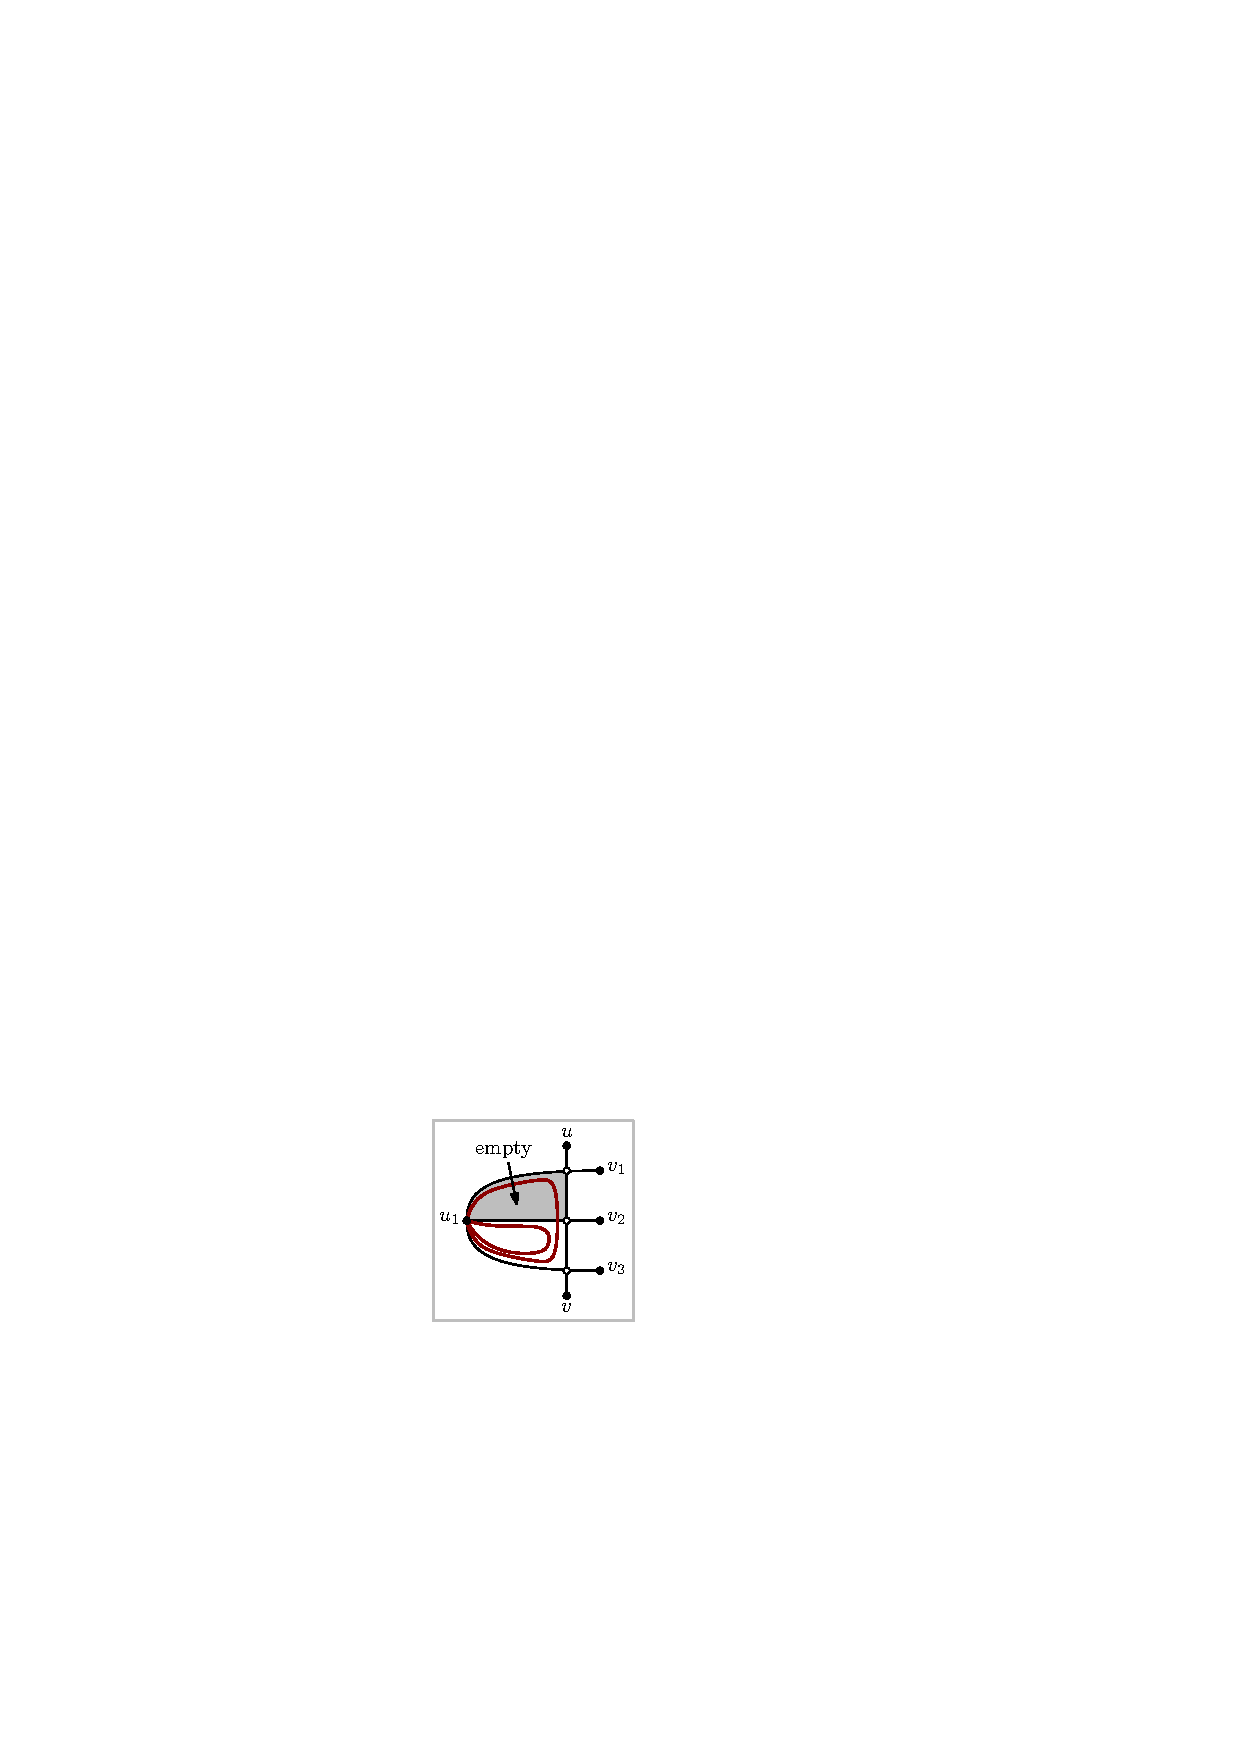
\includegraphics[width=\textwidth,page=1]{images/3planar_small_faces}
        \subcaption{~}\label{fig:3_planar_small_faces_example}
    \end{minipage}
    \begin{minipage}[b]{.24\textwidth}
        \centering
        \includegraphics[width=\textwidth,page=2]{images/3planar_small_faces}
        \subcaption{~}\label{fig:3_planar_small_faces_conf}
    \end{minipage}
    \begin{minipage}[b]{.24\textwidth}
        \centering
        \includegraphics[width=\textwidth,page=3]{images/3planar_small_faces}
        \subcaption{~}\label{fig:3_planar_small_faces_conf_middle_a}
    \end{minipage}
		\begin{minipage}[b]{.24\textwidth}
        \centering
        \includegraphics[width=\textwidth,page=4]{images/3planar_small_faces}
        \subcaption{~}\label{fig:3_planar_small_faces_conf_middle_b}
    \end{minipage}
    \caption{%
    (a):~If the parallel edge $[u_1,u_1]$ is a\pe for edges $(u_2,v_2)$ and $(u_3,v_3)$ then it is also a \pe for edges $(u_1,v_1)$ and $(u_3,v_3)$.  (b)-(d):~Configuration of Lemma~\ref{lem:3_planar_small_faces}.}
    \label{fig:3_planar_small_faces}
\end{figure}

By Lemma~\ref{lem:3_planar_small_faces}, we have that any edge of $G$ that is crossed three times in $\Gamma(G)$ is a chord of an empty true-planar $s$-cycle for $6\leq s\leq9$. So, it remains to consider edges of $G$ that have at most two crossings in $\Gamma(G)$, i.e. propagated sets of crossing edges where every edge has at most two crossings. Note that we can not use directly  Lemma~\ref{lem:2_planar_small_faces}, since its proof is based on the fact that optimal $2$-planar graphs have at most $5n-10$ edges, however, we can formulate its analogue lemma as follows:
\begin{lemma}
Let $\Gamma(G)$ be an almost-simple PMCM $3$-planar drawing of an optimal $3$-planar graph $G$ on $n$ vertices. Let $S$ be a propagated set of crossing edges where every edge has at most two crossings. Then edges of $S$ are chords of a true-planar $5$-cycle in $\Gamma(G)$, that contains no vertices in its interior. 
\label{lem:3_planar_small_faces_2}
\end{lemma}
\begin{proof}
We distinguish two cases depending on whether $S$ contains an edge with two crossings or not. Suppose first that this is not the case. Then all edges of $S$ have at most one crossing. Let $e\in S$ crossing with $e'\in S$. Clearly $S=\left\{e,e'\right\}$. The four endpoints of edges $e$ and $e'$ define a \pp $\mathcal{C}_4$ on $4$ vertices, as in Figure~\ref{fig:3_planar_one_crossing_before} and there are no other edges passing through the interior of $\mathcal{C}_4$. We proceed by removing edges $e$ and $e'$ and replace them with the $3$-planar pattern of Figure~\ref{fig:3_planar_one_crossing_after}. The derived graph $G'$ has $n'=n+1$ vertices and $m'=m-2+8$ edges, where $n$ and $m$ are the number of vertices and edges of $G$ respectively. Then, $G'$ is $3$-planar and has $m'=5.5n'-10.5>5.5n'-11$ edges; a contradiction to the optimality of $G$.

Now, assume that there exists an edge $e\in S$, where $e=(u,v)$ crossing with two edges $e_1=(u_1,v_1)$ and $e_2=(u_2,v_2)$. By Lemma~\ref{lem:3_planar_independent} edges $e_1$ and $e_2$ are not independent edges. Following the proof of Lemma~\ref{lem:2_planar_small_faces} we can find:
\begin{enumerate}
\item  a \pp on five vertices whose boundary edges define a true planar $5$-cycle with $e$ as a chord, or,
\item a \pp $\mathcal{C}_6$ on six vertices with at most $6$ edges passing through its interior. In this case, we remove all edges with an edge-segment in the set of passing-through segments of $\mathcal{C}_6$ and use the $3$-planar pattern of Figure~\ref{fig:6gon} that gives $8$ edges in drawn in the interior of $\mathcal{C}_6$. The derived graph clearly has more edges than $G$, contradicting its optimality.
\end{enumerate}
\end{proof}

\begin{figure}[htb]
    \centering
    \begin{minipage}[b]{.24\textwidth}
        \centering
        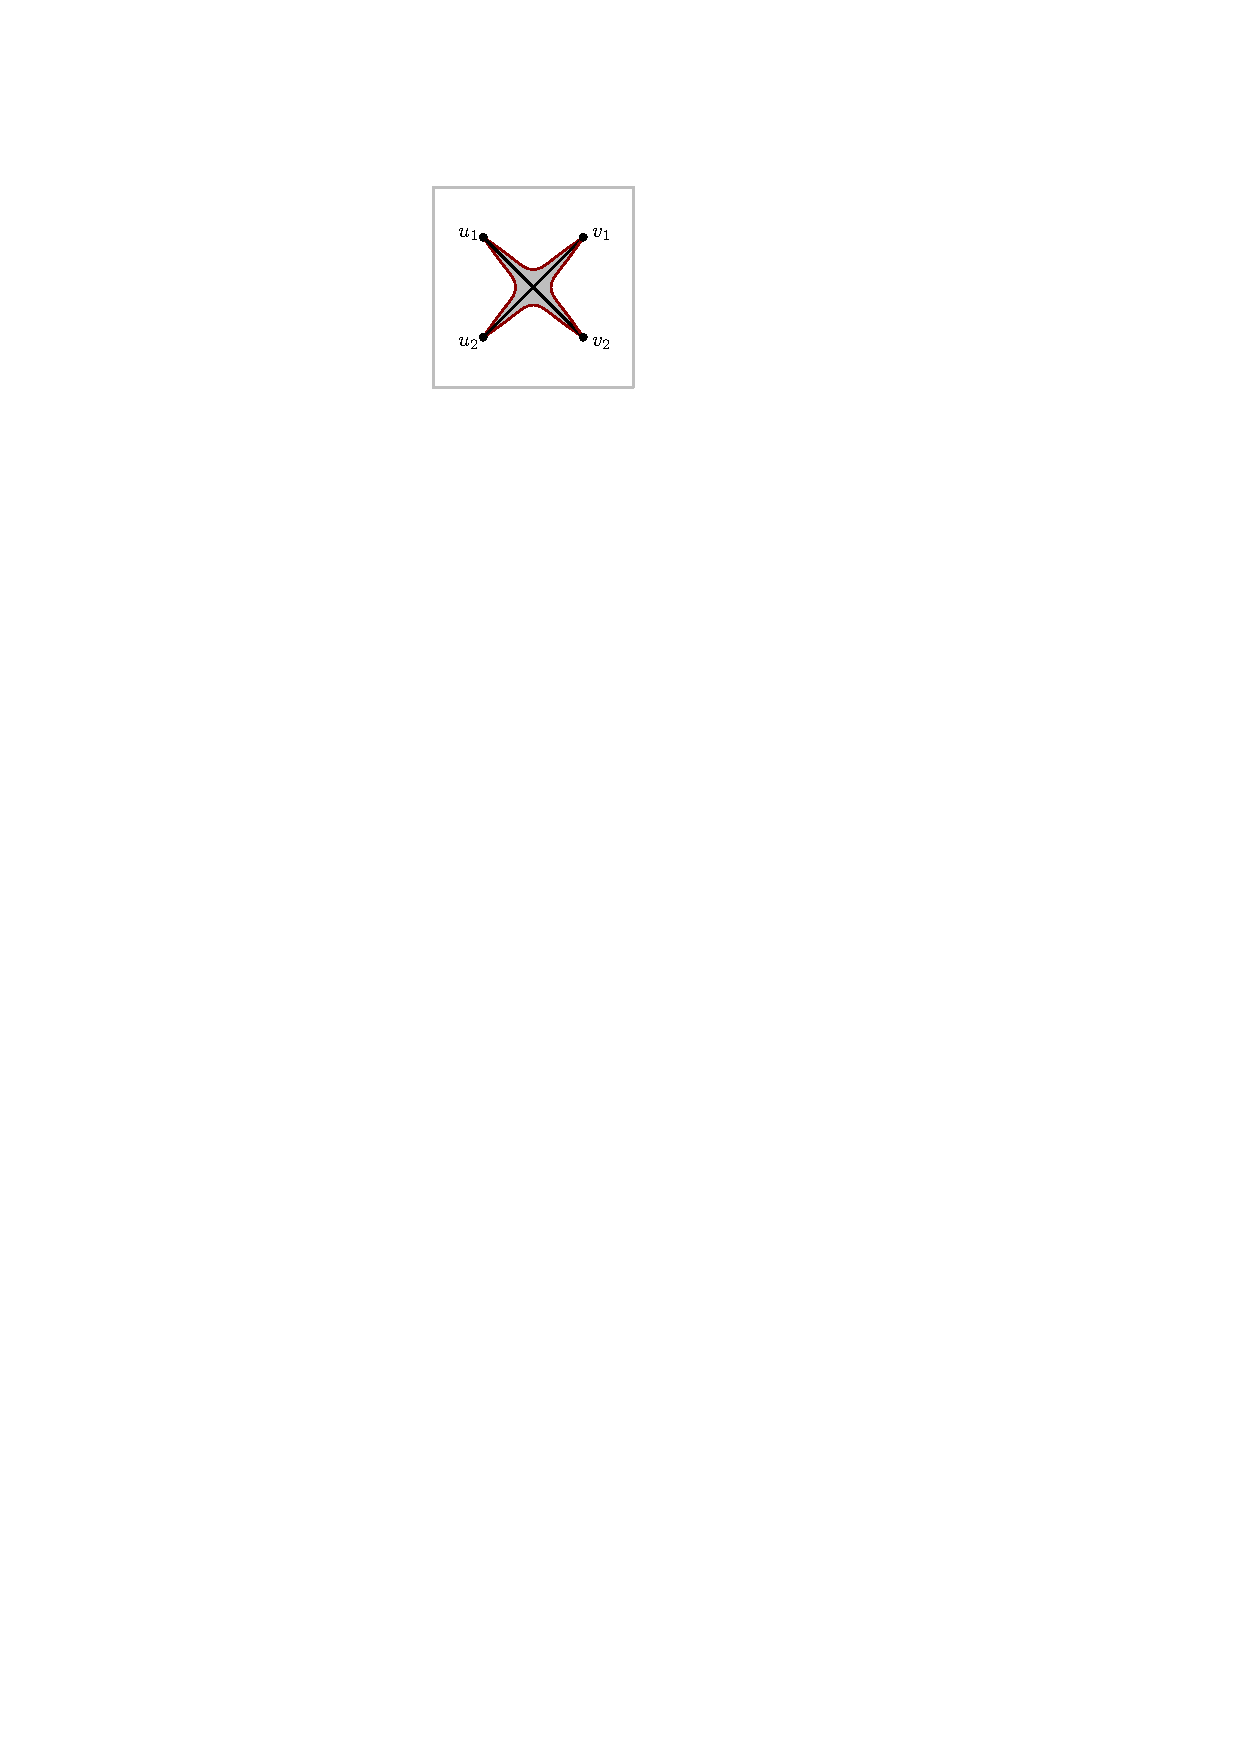
\includegraphics[width=\textwidth,page=1]{images/3planar_one_crossing}
        \subcaption{~}\label{fig:3_planar_one_crossing_before}
    \end{minipage}
    \begin{minipage}[b]{.24\textwidth}
        \centering
        \includegraphics[width=\textwidth,page=2]{images/3planar_one_crossing}
        \subcaption{~}\label{fig:3_planar_one_crossing_after}
    \end{minipage}
		\begin{minipage}[b]{.24\textwidth}
        \centering
        \includegraphics[width=\textwidth,page=3]{images/3planar_one_crossing}
        \subcaption{~}\label{fig:3_planar_triangle}
    \end{minipage}
    \caption{%
    (a)-(b):~Configurations used in Lemma~\ref{lem:3_planar_small_faces_2}. (c):~Configuration used in Lemma~\ref{lem:3_planar_triangle}}.
    \label{fig:3_planar_one_crossing_1}
\end{figure}

\begin{lemma}
Let $\Gamma(G)$ be an almost-simple PMCM $3$-planar drawing of an optimal $3$-planar graph $G$ on $n$ vertices. There is no true planar $3$-cycle without vertices in its interior. 
\label{lem:3_planar_triangle}
\end{lemma}
\begin{proof}
Suppose that there exists a true planar $3$-cycle in $\Gamma(G)$ without vertices in its interior. Then we can add a vertex in the interior of this cycle, and $6$ edges by using the $3$-planar pattern of Figure~\ref{fig:3_planar_triangle}. The derived graph $G'$ has $n'=n+1$ vertices and $m'=m+6$ edges, where $n$ and $m$ are the number of vertices and edges of $G$ respectively. Then, $G'$ is $3$-planar and has $m'=5.5n'-10.5>5.5n'-11$ edges; a contradiction.
\end{proof}


By combining Lemmas~\ref{lem:3_planar_small_faces}, \ref{lem:3_planar_small_faces_2} and \ref{lem:3_planar_triangle} the following is straightforward:
 
\begin{corollary}\label{cor:3_planar_faces_general}
The true planar structure $\Pi(G)$ of an almost-simple PMCM $3$-planar drawing of an optimal $3$-planar graph $G$ on $n$ vertices contains faces of length at least $5$ and at most $9$.
\end{corollary}

 
 Now we are ready to prove the main property of almost-simple PMCM $3$-planar drawings of optimal $3$-planar graphs.
 
 \begin{lemma}\label{lem:3_planar_faces_final}
  The true planar structure $\Pi(G)$ of an almost-simple PMCM $3$-planar drawing of an optimal $3$-planar graph $G$ on $n$ vertices contains only faces of length $6$.
 \end{lemma}

 \begin{proof}
  Let $e_{TP}$ be the total number of true planar edges of $G$. By Euler's formula we have that
  
  \begin{equation}
   e_{TP}+2=n+f
  \end{equation}
  
  where $f$ is the total number of faces of $G_{TP}$. Let $s_i$ be the number of faces of $G_{TP}$ of length $i$. By Corollary~\ref{cor:3_planar_faces_general} we have that $5\leq i\leq 9$. Hence,
  
  \begin{equation}
   f=s_5+s_6+s_7+s_8+s_9
  \end{equation}

  Also, by counting the edges of all faces of $G_{TP}$ we have that
  
  \begin{equation}
   2e_{T}=5s_5+6s_6+7s_7+8s_8+9s_9
  \end{equation}

  On the other hand for the number of crossing edges of $G$, say $e_{CR}$, by Lemmas~\ref{lem:no-of-edges} and \ref{lem:3_planar_small_faces_2} we have
  
  \begin{equation}
   e_{CR}=5s_5+8s_6+9s_7+11s_8+14s_9
  \end{equation}

  Hence, for the total number of edges of $G$ we have 
	%\todo{rewrite the equations}
  

  $\begin{array}{ll}
   |E(G)|= & 5.5n-11\\
    \Rightarrow &e_{TP}+e_{CR}= 5.5n-11\\
    \Rightarrow &e_{TP}+e_{CR}= 5.5(e_{TP}-f)\\
    \Rightarrow &2e_{CR}= 9e_{TP}-11f\\
    \Rightarrow &10s_5+16s_6+18s_7+22s_8+28s_9 = 4.5(5s_5+6s_6+7s_7+8s_8+9s_9)\\
   &-11(s_5+s_6+s_7+s_8+s_9)\\
    \Rightarrow &10s_5+16s_6+18s_7+22s_8+28s_9=11s_5+16s_6+20.5s_7+25s_829.5s_9\\
    \Rightarrow &0= s_5+2.5s_7+3s_8+1.5s_9\\
   \Rightarrow &0=s_5=s_7=s_8=s_9
  \end{array}$

The last equation implies that there are only faces of length $6$, hence $f=f_6$.
 \end{proof}

Recall that at the beginning of this section we made the assumption that $\Gamma(G)$ is almost-simple, i.e. there is no pair of edges that cross twice in the drawing $\Gamma(G)$. In the following, we prove that in any PMCM drawing of an optimal $3$-planar graph $G$ on $n$ vertices there are no such pairs of edges.
 %By Lemma~\ref{lem:2_planar_faces} we can characterize all maximal $2$-planar graphs. Since the true planar subgraph of such a graph contains only faces of length $5$, we can start with a $5$-tiling of the plane. Now in the interior of every face of length $5$, we can add all  $5$ missing edges.

\begin{lemma}
Let $\Gamma(G)$ be a PMCM $3$-planar drawing of an optimal $3$-planar graph $G$ on $n$ vertices. Then $\Gamma(G)$ is almost-simple.
%There is no pair of edges that cross twice in $\Gamma(G)$. 
\label{lem:3_planar_cross_twice}
\end{lemma}

\begin{proof}
For a proof by contradiction, suppose that there exist edges $(u_1,v_1)$ and $(u_2,v_2)$ that cross twice at crossing points $c_1$ and $c_2$ as in Figure~\ref{fig:3_planar_cross_twice_general}. Consider the bounded region $\mathcal{R}_{IN}$ defined by $(c_1,c_2)$ segment of edges $(u_1,v_1)$ and $(u_2,v_2)$. Let $V_{IN}\subset V(G)$ be the subset of vertices of $G$ that lie in the interior of $\mathcal{R}_{IN}$. By Lemma~\ref{lem:crossing_twice} $|V_{IN}|\geq 1$. Also, since edges $(u_1,v_1)$ and $(u_2,v_2)$ have already two crossings, there exist at most one edge $e'_1$ and an edge $e'_2$ that cross with $(u_1,v_1)$ and $(u_2,v_2)$ respectively. Since $G$ is connected \todo{mention that G is connected} at least one of $e'_1$ or $e'_2$ has an endpoint in $V_{IN}$. Suppose w.l.o.g. that $e'_1$ is an edge incident to vertex $w$, where $w\in V_{IN}$. Note that vertices $u_1$-$u_2$ define a corner pair of vertices and therefore the corner edge $[u_1,u_2]$ is a \pe (refer to the upper red edge of Figure~\ref{fig:3_planar_cross_twice_region}). Also, since $V_{IN}$ is not empty, another \pe $[u_1,u_2]$ exists (refer to the lower red edge of Figure~\ref{fig:3_planar_cross_twice_region}), such that the bounded region defined by these two \pes contains only $V_{IN}$ in its interior. Let $E_w$ be the set of edges of $G$ that have both endpoints in $V_{IN}$ and cross with edge $e'_1$ in the drawing $\Gamma(G)$ (refer to the light red edge of Figure~\ref{fig:3_planar_cross_twice_region}). Denote by $m_w$ the number of edges in $E_w$. Since $e'_1$ already crosses with edge $(u_1,v_1)$, $m_w\leq 2$. Now we distinguish two cases depending on whether $|V_{IN}|=1$ or $|V_{IN}|\geq 2$.

In the first case, we have that $V_{IN}=\left\{w\right\}$ and edge $E_w$ must be empty, i.e. $m_w=0$. We proceed by removing edges $(u_1,v_1)$, $(u_2,v_2)$ and any other edge that crosses with them, and replace them with the $3$-planar pattern of Figure\ref{fig:3_planar_cross_twice_single}. We add a vertex, say $x$ and true planar edges $(u_1,x)$ and $(x,w)$. Vertices $u_1$, $x$, $w$, $x$, $u_1$, $u_2$ define a \pp $\mathcal{P}$ on six vertices (grey shaded in Figure~\ref{fig:3_planar_cross_twice_single}). In the interior of $\mathcal{P}$ we can add $8$ edges by using the $3$-planar pattern of Figure~\ref{fig:6gon}. The derived graph, say $G'$, has $n'=n+1$ vertices and at least $m'=m-4+10$ edges, where $n$ and $m$ are the number of vertices and edges of $G$ respectively. Hence $G'$ has $m'\geq 5.5n'-10.5>5.5n'-11$, i.e. more edges than allowed, a clear contradiction.

In the second case, where $|V_{IN}|\geq 2$, we proceed by removing edges $(u_1,v_1)$, $(u_2,v_2)$, any other edge that crosses with them, and edges of $E_w$, i.e. we remove at most $4+m_w$ edges. We replace them with the $3$-planar pattern of Figure\ref{fig:3_planar_cross_twice_main}. We add a vertex, say $x$, true planar edge $(u_1,x)$ and two true planar non homotopic parallel edges $(x,w)$ that contain only vertices $V_{IN}-\left\{w\right\}$ in the bounded region that they define. As in the previous case, vertices $u_1$, $x$, $w$, $x$, $u_1$, $u_2$ define a \pp $\mathcal{P}$ on six vertices (grey shaded in Figure~\ref{fig:3_planar_cross_twice_main}). In the interior of $\mathcal{P}$ we can add $8$ edges by using the $3$-planar pattern of Figure~\ref{fig:6gon}. Finally, we can add a loop (if it is not already present in $\Gamma(G)$), say $\ell_w$,  at vertex $w$ containing all vertices of $V_{IN}-\left\{w\right\}$ (red loop of Figure~\ref{fig:3_planar_cross_twice_main}). The derived graph, say $G'$, has $n'=n+1$ vertices and at least $m'\geq m-(4+m_w)+11$ edges, where $n$ and $m$ are the number of vertices and edges of $G$ respectively. Hence $G'$ has $m'\geq 5.5n'-9.5-m_w$. Since $G'$ is $3$-planar $m'\leq 5.5n'-11$ also holds. By combining the two equations we have that $5.5n'-9.5-m_w\leq 5.5n'-11\Rightarrow 1.5\leq m_w$. Recall that $m_w\geq 2$, hence it must be the case that $m_w=2$ and $m'= m-(4+m_w)+11$. However, the last equality holds only in the case where the loop $\ell_w$ already exists in $G$. Now, note that any edge of $E_w$ crosses twice with loop $\ell_w$, which implies that $\ell_w$ has at least $4$ crossings, a clear contradiction.
\end{proof}

\begin{figure}[htb]
    \centering
    \begin{minipage}[b]{.24\textwidth}
        \centering
        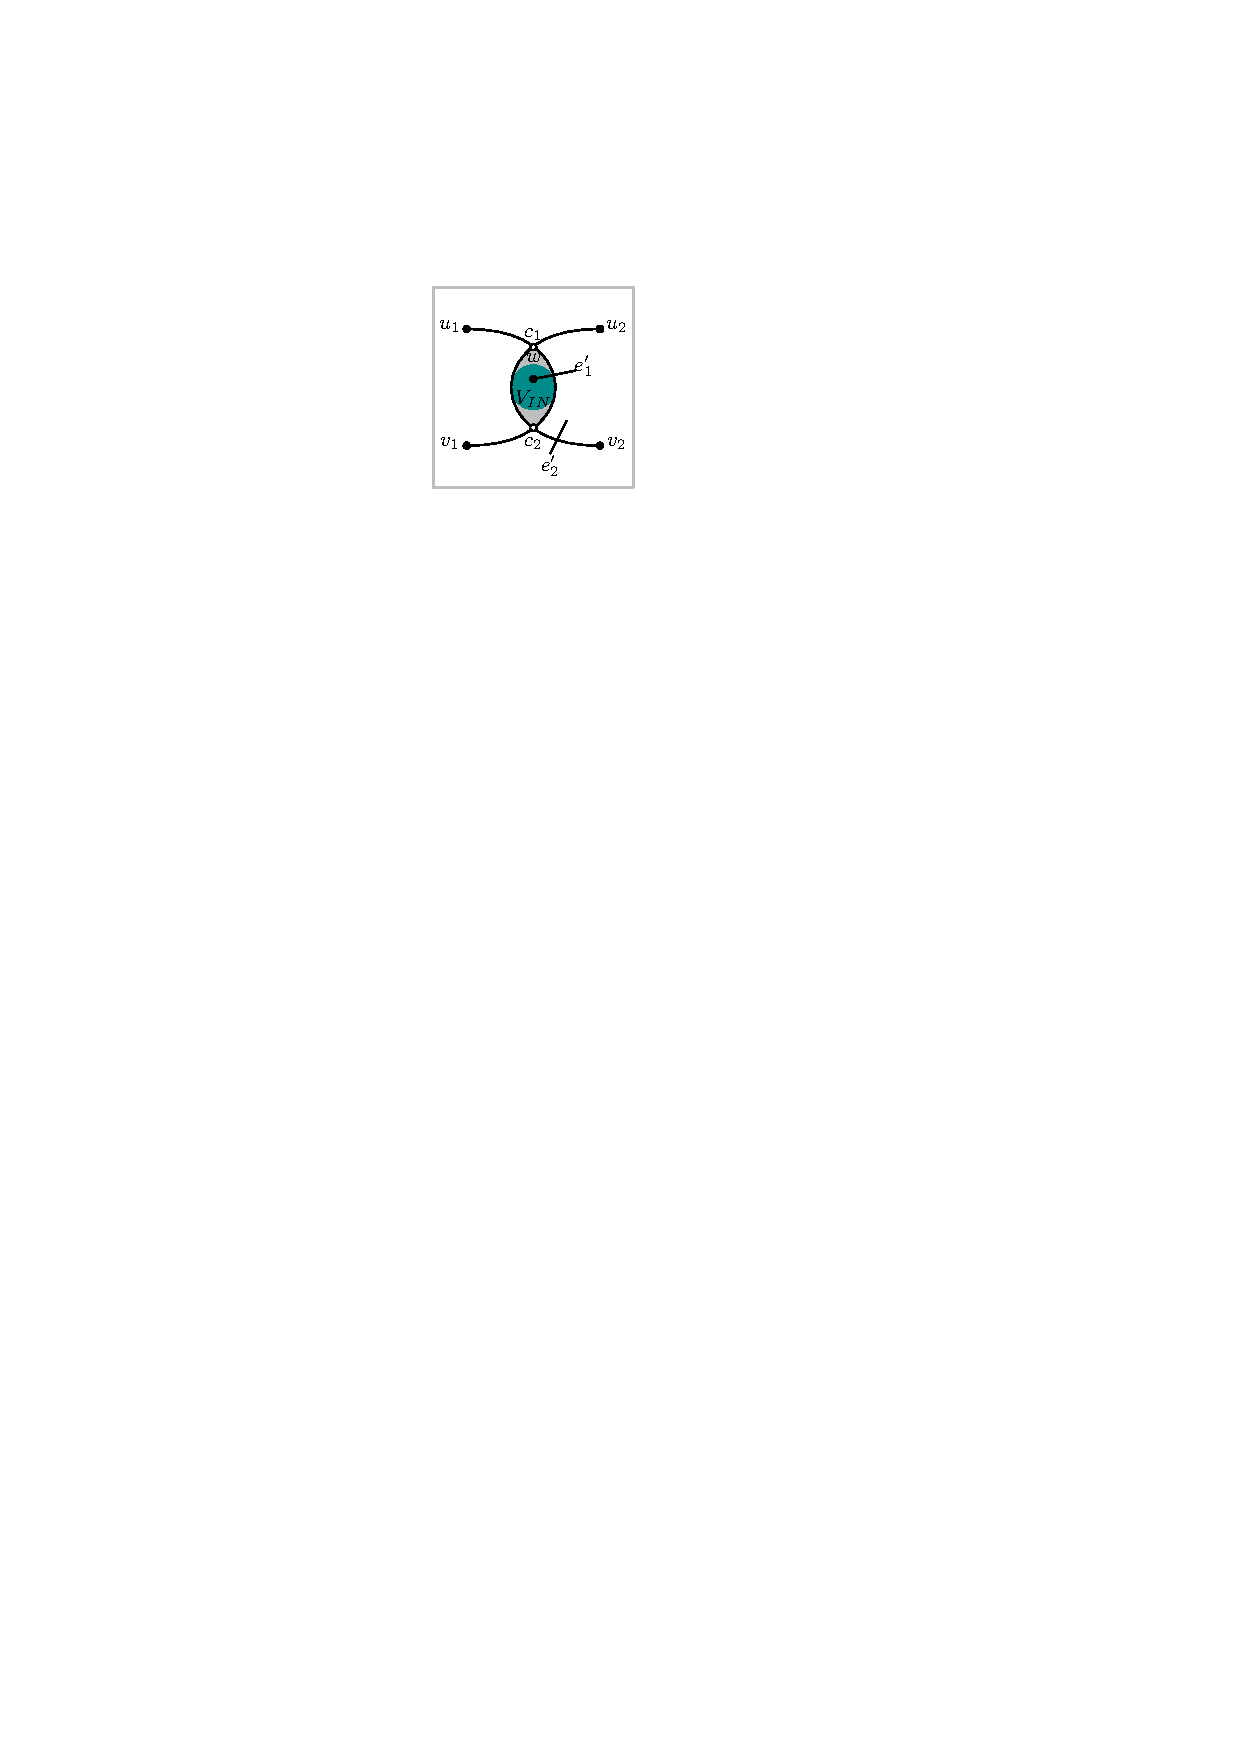
\includegraphics[width=\textwidth,page=1]{images/3_planar_cross_twice}
        \subcaption{~}\label{fig:3_planar_cross_twice_general}
    \end{minipage}
    \begin{minipage}[b]{.24\textwidth}
        \centering
        \includegraphics[width=\textwidth,page=2]{images/3_planar_cross_twice}
        \subcaption{~}\label{fig:3_planar_cross_twice_region}
    \end{minipage}
		\begin{minipage}[b]{.24\textwidth}
        \centering
        \includegraphics[width=\textwidth,page=3]{images/3_planar_cross_twice}
        \subcaption{~}\label{fig:3_planar_cross_twice_single}
    \end{minipage}
    \begin{minipage}[b]{.24\textwidth}
        \centering
        \includegraphics[width=\textwidth,page=4]{images/3_planar_cross_twice}
        \subcaption{~}\label{fig:3_planar_cross_twice_main}
    \end{minipage}
    \caption{%
    (a)-(d):~Configurations used in Lemma~\ref{lem:3_planar_cross_twice}.
    \label{fig:3_planar_one_crossing_2}}
\end{figure}

By combining Lemmas~\ref{lem:3_planar_faces_final} and \ref{lem:3_planar_cross_twice}, we can characterize all optimal $3$-planar graphs:


 By Lemma~\ref{lem:3_planar_cross_twice} we have that Lemma~\ref{lem:3_planar_faces_final} holds for all maximal $3$-planar graphs. Since the true planar subgraph of such a graph contains only faces of length $6$, we can start with a $6$-tiling of the plane\todo{rephrase}. Now in the interior of every face of length $6$, we can add all  $8$ missing edges using the $3$-planar pattern of Figure~\ref{fig:6gon}.
 %By Lemma~\ref{lem:3_planar_faces_final} we can characterize all maximal $3$-planar graphs. Since the true planar subgraph of such a graph contains only faces of length $6$, we can start with a $6$-tiling of the plane. Now in the interior of every face of length $6$, we can add all  $8$ missing edges.

